\chapter{Fundamental teórico}
\section{Estudo de coorte}
A palavra coorte tem origem no latim \textit{cohors}. Esse termo era utilizado para nomear uma unidade militar do Império Romano, que compunha uma legião. Pode ser considerada equivalente ao conceito moderno de batalhão. No contexto científico, uma coorte pode ser definida como um grupo de pessoas que possuem uma característica ou experiência em comum. Coortes podem ser estabelecidas com vários propósitos. Um deles é a análise de grupos dentro de um determinado domínio, como em estudos econométricos, epidemiológicos e demográficos. Dentro das metodologias utilizadas para explorar uma questão específica estão os estudos observacionais. O que diferencia os estudos de caráter observacional de outros estudos é a realização de intervenções. Nesses estudos, os pesquisadores não interferem nos fenômenos estudados, apenas os observam, fazendo com que a variável considerada não esteja sob controle \autocite{Song2010}.

\begin{figure}[h]
\caption{Tipos de estudos observacionais}
\centering
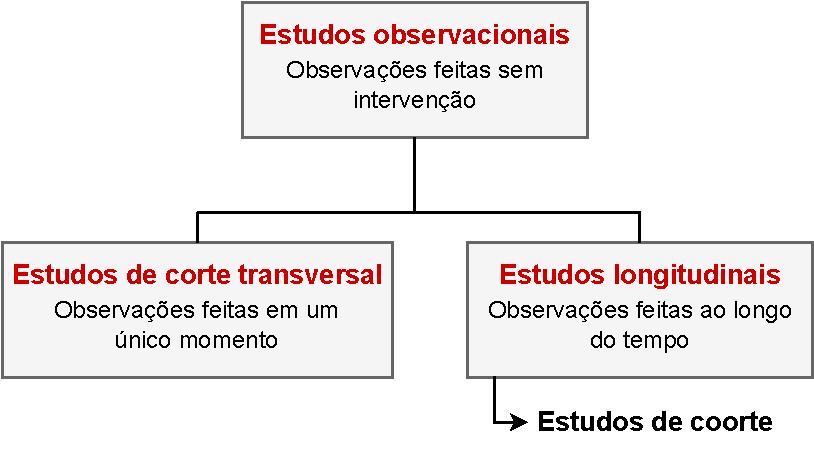
\includegraphics{figuras/diagrama-estudos-observacionais.pdf}
\end{figure}


Estudos observacionais podem ser divididos de acordo com o período de coleta de dados. Quando as observações são feitas em um momento específico, coletando dados em um curto intervalo de tempo, chamamos de estudo de corte transversal. Eles são úteis para observar o estado e as condições atuais dos participantes, sem que haja um acompanhamento dos mesmos \autocite{Zangirolami-Raimundo2018}. Alguns exemplos de estudos que seguem essa estrutura no Brasil são o \href{https://www.ibge.gov.br/estatisticas/sociais/trabalho/22827-censo-demografico-2022.html?=&t=o-que-e}{Censo Demográfico}, realizado a cada 10 anos pelo IBGE, e o \href{https://www.gov.br/inep/pt-br/areas-de-atuacao/pesquisas-estatisticas-e-indicadores/censo-escolar}{Censo Escolar}, realizado anualmente pelo INEP. 

Já quando os indivíduos são acompanhados por longos períodos de tempo, os estudos são classificados como longitudinais. São realizadas coletas de dados contínuas ou repetidas em intervalos regulares, como dias, meses e anos. Como os dados levam em consideração um grupo pré-definido, é possível ajustar os métodos estatísticos para mudanças observadas ao longo do tempo para o grupo como um todo ou para sujeitos específicos \autocite{Caruana2015}. Temos como exemplos o \href{https://www.b3.com.br/pt_br/market-data-e-indices/indices/indices-amplos/ibovespa.htm}{índice Bovespa}, disponibilizado pela B3 e \href{https://www.bcb.gov.br/controleinflacao/taxaselic}{taxa Selic}, disponibilizada pelo Banco Central.

Os estudos de coorte são um tipo de estudo longitudinal que leva em consideração uma segmentação específica da população, que é a coorte. Um exemplo de estudo de coorte é a observação do desenvolvimento de doenças em uma população. A amostra populacional pode ser dividida em duas coortes: a coorte 1, de expostos à doença e a coorte 2, de não expostos. Assim, é possível comparar a ocorrência da doença entre os grupos. Estudos de coorte podem ser conduzidos de duas maneiras principais: 

\begin{itemize}
  \item Nos estudos prospectivos, os indivíduos são acompanhados do início do estudo, no presente, durante um período de tempo, para analisar os dados recolhidos no futuro;
  \item Nos estudos retrospectivos, os dados são coletados e mensurados no passado, acompanhados por um determinado período de tempo, para a realização de uma análise no presente.
\end{itemize}

Na área da educação, estudos de coorte podem utilizados para analisar como questões específicas impactam sujeitos inseridos no sistema educacional, como professores, estudantes e outros envolvidos. \citet{Bjorkenstam993} investigou a associação da performance escolar com taxas de suicídio em estágios posteriores da vida, utilizando uma coorte de nascidos entre 1972 e 1981 na Suécia. Outro exemplo foi o trabalho de \citet{Ensminger1992}, que examinou os caminhos de desenvolvimento de uma coorte de estudantes negros de uma escola de Chicago entre 1966 e 1977. No sentido dessa pesquisa, pode-se delimitar uma coorte como um grupo de estudantes que estão inseridos no mesmo ambiente escolar. Eles interagem entre si, podem desenvolver relacionamentos e compartilhar experiências. A realização de estudos de coorte educacionais, em particular os retrospectivos, como é o atual, é facilitada pela disponibilização de dados públicos de diferentes abrangências. No Brasil, há a inicativa do \href{https://dados.gov.br/home}{Portal Brasileiro de Dados Abertos}, com dados a nível federal e local de múltiplas áreas. 


\section{Estratégias empíricas: Variações idiossincráticas na composição de gênero}
\label{sec:variacoes}
Variações idiossincráticas podem ser definidas como particularidades e diferenças individuais únicas que podem influenciar resultados ou comportamentos. Esses fatores comuns ou gerais que afetam um grupo de indivíduos também influenciam os sistemas nos quais estes estão inseridos \autocite{Meister1991}. Essas variações podem ser diversas, abrangendo uma ampla gama de características, experiências e situações pessoais. Alguns exemplos de variações são:

\begin{itemize}
  \item \textbf{Contexto pessoal:} Dinâmica familiar, status socioeconômico, crenças, \textit{background} cultural, valores familiares;
  \item \textbf{Carreira:} Aspirações e objetivos profissionais, experiência prévia de trabalho, habilidades técnicas; 
  \item \textbf{Educação:} Qualidade escolar, atividades extracurriculares, exposição prematura a tópicos avançados. 
\end{itemize}

Por serem altamente individualizadas e frequentemente envolverem múltiplos fatores, é um desafio conduzir uma pesquisa que isole e entenda o impacto de fatores específicos, como o efeito de pares. O efeito de pares (do inglês \textit{peer effect}) se refere à influência e impactos que indivíduos dentro do círculo próximo (familiar, social ou educacional) têm nas suas decisões e comportamentos. Um trabalho muito relevante no entendimento dos efeitos sociais do grupo que uma pessoa se insere é o de \citet{Manski1993}. Ele aponta a existência de efeitos de pares correlatos, que são comportamentos similares em pessoas do mesmo grupo por conta da semelhança de características individuais ou ambientes institucionais.

Isso é especialmente importante no contexto educacional, já que estudantes do ensino médio compartilham o ambiente escolar durante sua formação. Inseridos em classes diversificadas, eles devem conviver diariamente com outros adolescentes por uma parte relevante de suas vidas. Os colegas de escola podem ser uma importante força social não só na performance acadêmica, mas também nas aspirações profissionais e decisões de seguir uma área específica \autocite{Tang2008}.  

A literatura observa que os pares têm grande relevância em comportamentos, escolhas e resultados educacionais \autocite{Sacerdote2014, Zimmerman2003}. Para entender melhor esse efeito, é importante considerar como estão estruturados os grupos de referências de estudantes, já que eles são altamente vulneráveis à influência uns dos outros pela exposição contínua e proximidade. Os efeitos dos pares podem se apresentar tanto de maneira positiva, quanto negativa, que se refletem em pontuações de prova, motivação e hábitos de estudo, por exemplo. Uma maneira de fazer isso é através da observação da composição das turmas, isto é, como diferentes distribuições dos pares nas classes de aula afetam os alunos.

Um importante precursor dessas observações é o estudo de \citet{Hoxby-2000}. Ela identificou e mensurou a existência de efeitos dos pares em coortes escolares que diferem na composição de fatores específicos, como o gênero. Seus resultados sugerem que um grupo de pares com maioria feminina eleva as pontuações de meninos e meninas em matemática e leitura.

Nesse sentido, múltiplos trabalhos exploram o problema com uma metodologia similar, denominada de variações idiossincráticas na composição de gênero \autocite{Schne2019, Lavy2011, Schneeweis2012, Brene2020, Borges2021}. Eles utilizam estratégicas empíricas para levantar hipóteses que ajudem a estabelecer um modelo econométrico para investigar os efeitos de gênero entre os pares. 

%\citet{Schne2019} sugere que a composição de gênero pode afetar escolhas educacionais por meio do impacto em seu desempenho, como boa performance em matemática e ciências levar a escolhas de cursos STEM. Outra possibilidade é através da influência dos pares em associar escolhas à identidade de gênero, que pode levar a uma conformidade a papéis tradicionais de gênero.

Os modelos econométricos, apesar de semelhantes, diferem-se por conta de serem estimados utilizando conjuntos de dados educacionais de diferentes países (Noruega, Israel, Áustria, Dinamarca e Brasil), que se configuram em sistemas de ensino distintos, bem como se apoiam em outros recursos, como registros demográficos. Além disso, são consideradas diferentes etapas da educação básica, como anos iniciais e finais do fundamental e médio. Uma lista não exaustiva de variáveis analisadas inclui parcela de estudantes do gênero feminino observadas na coorte escolar, características individuais e escolares e efeitos fixos de escola e coorte. 

Como parte da nossa metodologia se propõe a analisar o efeito da composição de gênero nas escolhas de graduação, utilizaremos como referência o trabalho de \cite{Borges2021}, que se volta para coortes de escolas de ensino médio brasileiras, um contexto similar ao nosso. Para esse propósito, ela emprega dados do Censo Escolar e do vestibular da Universidade Estadual de Campinas (UNICAMP). As definições teóricas apresentadas, assim como a equação definida, foram extraídas do capítulo \textit{Gender peer effects on major choice} \autocite{Borges2021}. 

\subsection{Efeitos de gênero em escolhas de graduação}
A hipótese da estratégia empírica é de que o efeito de pares tem um papel significativo na influência das escolhas do curso de graduação. Pais e alunos podem escolher suas turmas potenciais, que pode ser um problema por conta do viés da auto-seleção (\textit{self-selection bias}). Apesar das escolhas pessoais das famílias, elas não conseguem prever corretamente as variações coorte a coorte na composição de gênero dos estudantes, que seguem processos aleatórios. Assim, explorando a variação idiossincrática de coortes na proporção de alunas, temos a estimação do seguinte modelo econométrico, onde \textit{i} indexa estudante, \textit{e} escolas, \textit{c} coorte e \textit{t} ano do vestibular:

\begin{equation}
\begin{split}
y_{iect} = \gamma_0 + \beta_1 \textit{Feminino}_i + \beta_2 \textit{Prop\_FemEM}_{iec} + \\ \beta_3 \textit{Feminino}_i \times \textit{Prop\_FemEM}_{iec} + \alpha_e + \alpha_t + X_i \omega + Z_{ec} \delta + \gamma_{et} + \epsilon_{iect}
\end{split}
\end{equation}

A equação representa um modelo de regressão para estimar o impacto de alguns fatores na variável dependente $y_{iect}$. Ela é composta por:

\begin{itemize}
  \item $\textit{Feminino}_i$, indicador de gênero;
  \item $\textit{Prop\_FemEM}_{iec}$, proporção de colegas do gênero feminino na escola \textit{e} no ano de conclusão do ensino médio \textit{c};
  \item $\alpha_e$, efeitos fixos da escola;
  \item $\alpha_t$, efeitos fixos do ano do vestibular;
  \item $X_i$, vetor de características individuais do aluno (notas do ENEM, idade, indicador de trabalho durante o ensino médio);
  \item $Z_{ec}$, variáveis da coorte escolar: tamanho da turma, proporção de alunos que frequentam aulas diurnas, idade média dos colegas;
  \item $\gamma_{et}$, tendência linear de tempo específica da escola;
  \item $\beta_1$, coeficiente de diferenças de gênero nas variáveis de resultados;
  \item $\beta_2$, coeficiente de efeitos de pares de gênero aplicáveis tanto a homens quanto a mulheres;
  \item $\beta_3$, coeficiente do impacto diferencial de mulheres terem uma proporção maior de colegas do sexo feminino.
\end{itemize}

As variáveis de resultado ($y_{iect}$) podem ser agrupadas de acordo com o objetivo principal. Para analisar se maiores proporções de colegas do sexo feminino durante o ensino médio influenciam a escolha de graduação das alunas, são consideradas duas variáveis: um indicador de área intensiva em matemática e física, outro de escolha de curso STEM.  Já para analisar o efeito das colegas do sexo feminino na composição de gênero de um curso, são mensurados se o curso tem maioria de mulheres (\textit{female-dominated}), homens (\textit{male-dominated}) ou é balanceado entre os gêneros (\textit{gender-balanced}) e a média de aplicantes do gênero feminino. Por fim, para analisar o impactos das colegas na probabilidade de escolher cursos competitivos, foram consideradas as médias de candidatos por vaga e de notas de corte.

De forma similar, utilizaremos a metodologia de \citet{Borges2021} para analisar os efeitos da composição de gênero das coortes de ensino médio nas opções de carreira dos estudantes, dessa vez numa perspectiva mais abrangente, que é proporcionada pelo conjunto de dados do SISU. Abordaremos com mais detalhes no \autoref{chap:metodologia} como isso será feito.